% Partie 3: l'héritage
\chapter{La maladie, la mort, l'héritage}

\section{La maladie}

\section{La mort}
\epigraph{%
J'suis snob... Encore plus snob que tout à l'heure\\%
Et quand je serai mort\\%
J'veux un suaire de chez Dior!%
}{\emph{J'suis snob}, Boris Vian}

\lettrine{J}e ne sais pas si \BV\ a été enterré dans un suaire de chez Dior,
comme il le réclamait dans sa chanson «J'suis snob»\ldots ça aurait été la
moindre des choses. Enfin, je ne suis pas tout à fait persuadé que Dior
ai développé une lighe de suaires. Ils auraient pu commencer avec celui
de Boris\ldots

\subsection{La malédiction}
L'ayant poursuivi dès sa création, \emph{J'irai cracher sur vos tombes}, à
l'origine une bonne blague, l'aura finalement achevé. Ironie finie, quand
on sait qu'il est mort d'une crise cardiaque lors de la première
projection d'une adaptation de son \oe{}uvre qu'il avait tout fait pour
qu'elle ne voie pas le jour. Las. Par une vengeance d'une bassesse inomable,
celle ci n'a pas attendu les premières minutes pour porter le coup fatal.

\subsection{Dans son \oe{}uvre}
Se sachant condamné, \BV\ vit à cent à l'heure, accomplissant plus en \nb{39} ans
d'éxistance que ce que l'on pourrait imaginer réaliser en \nb{80}. Son \oe{}uvre 
est bien sûr marquée par cett menace de moins en moins diffuse à mesure que 
les années passent, et que les problèmes de santé se multiplient. «Je ne
vivrai pas jusqu'à \nb{40} ans», a-t-il dit un jour. On en vient presque à
regretter tant de clairvoyance. Cependant, ses amis savaient que ses jours
étaient comptés. Ainsi, ils avaient conscience que chaque note qui sortait
de sa trompinette le rapprochait un peu plus de la tombe. Pourtant, il
s'efforcait de vivre, le plus intensément possible.

Sa mort ne venant pas par surprise --- seule la date exacte,
judicieusement choisie par le Sort, ça l'aurait probablement fait rire,
a été gardée secrète jusqu'au bout; il a eu le temps d'y réfléchir. Il y
fait référence dans beaucoup de ses textes. Voilà une petite sélection,
pour se faire une idée.

\subsubsection{Quand j'aurai du vent dans mon crâne}

Il s'agit d'une chanson (je ne peux malheureusement pas inclure dans ce document
la très bonne interprétation de Serge \bsc{Reggiani}, je vais donc simplement
en recommander fortement l'écoute) écrite en \nb{19}??, sur une musique de l'inénérable Serge \bsc{Gainsbourg}.

\begin{multicols}{2}
{\footnotesize
\settowidth{\versewidth}{Quand j'aurai du vent dans mon crâne}
\begin{verse}[\versewidth]
Quand j'aurai du vent dans mon crâne\\
Quand j'aurai du vert sur mes osses\\
P'tet qu'on croira que je ricane\\
Mais ça sera une impression fosse\\
Car il me manquera\\
Mon élément plastique\\
Plastique tique tique\\
Qu'auront bouffé les rats\\
Ma paire de bidules\\
Mes mollets mes rotules\\
Mes cuisses et mon cule\\
Sur quoi je m'asseyois\\
Mes cheveux mes fistules\\
Mes jolis yeux cérules\\
Mes couvre-mandibules\\
Dont je vous pourléchois\\
Mon nez considérable\\
Mon coeur mon foie mon râble\\
Tous ces riens admirables\\
Qui m'ont fait apprécier\\
Des ducs et des duchesses\\
Des papes des papesses\\
Des abbés des ânesses\\
Et des gens du métier\\
Et puis je n'aurai plus\\
Ce phosphore un peu mou\\
Cerveau qui me servit\\
A me prévoir sans vie\\
Les osses tout verts, le crâne venteux\\
Ah comme j'ai mal de devenir vieux.


\end{verse}
}
\end{multicols}

En parlant d'interprétation, je ne peux m'empêcher d'inclure ici la version
du dessinateur de bande dessinée Boulet, publiée sur son blog à l'occasion
de son trente-et-unième anniversaire. Un très bel hommage, respectant
d'après moi l'esprit de la chanson, à lire en fig. \ref{boulet}%
--- que j'ai malheureusement dû couper pour passer du format «Internet» au format «livre».

\begin{figure}[!htb]
\centering
\subfloat[][]{%
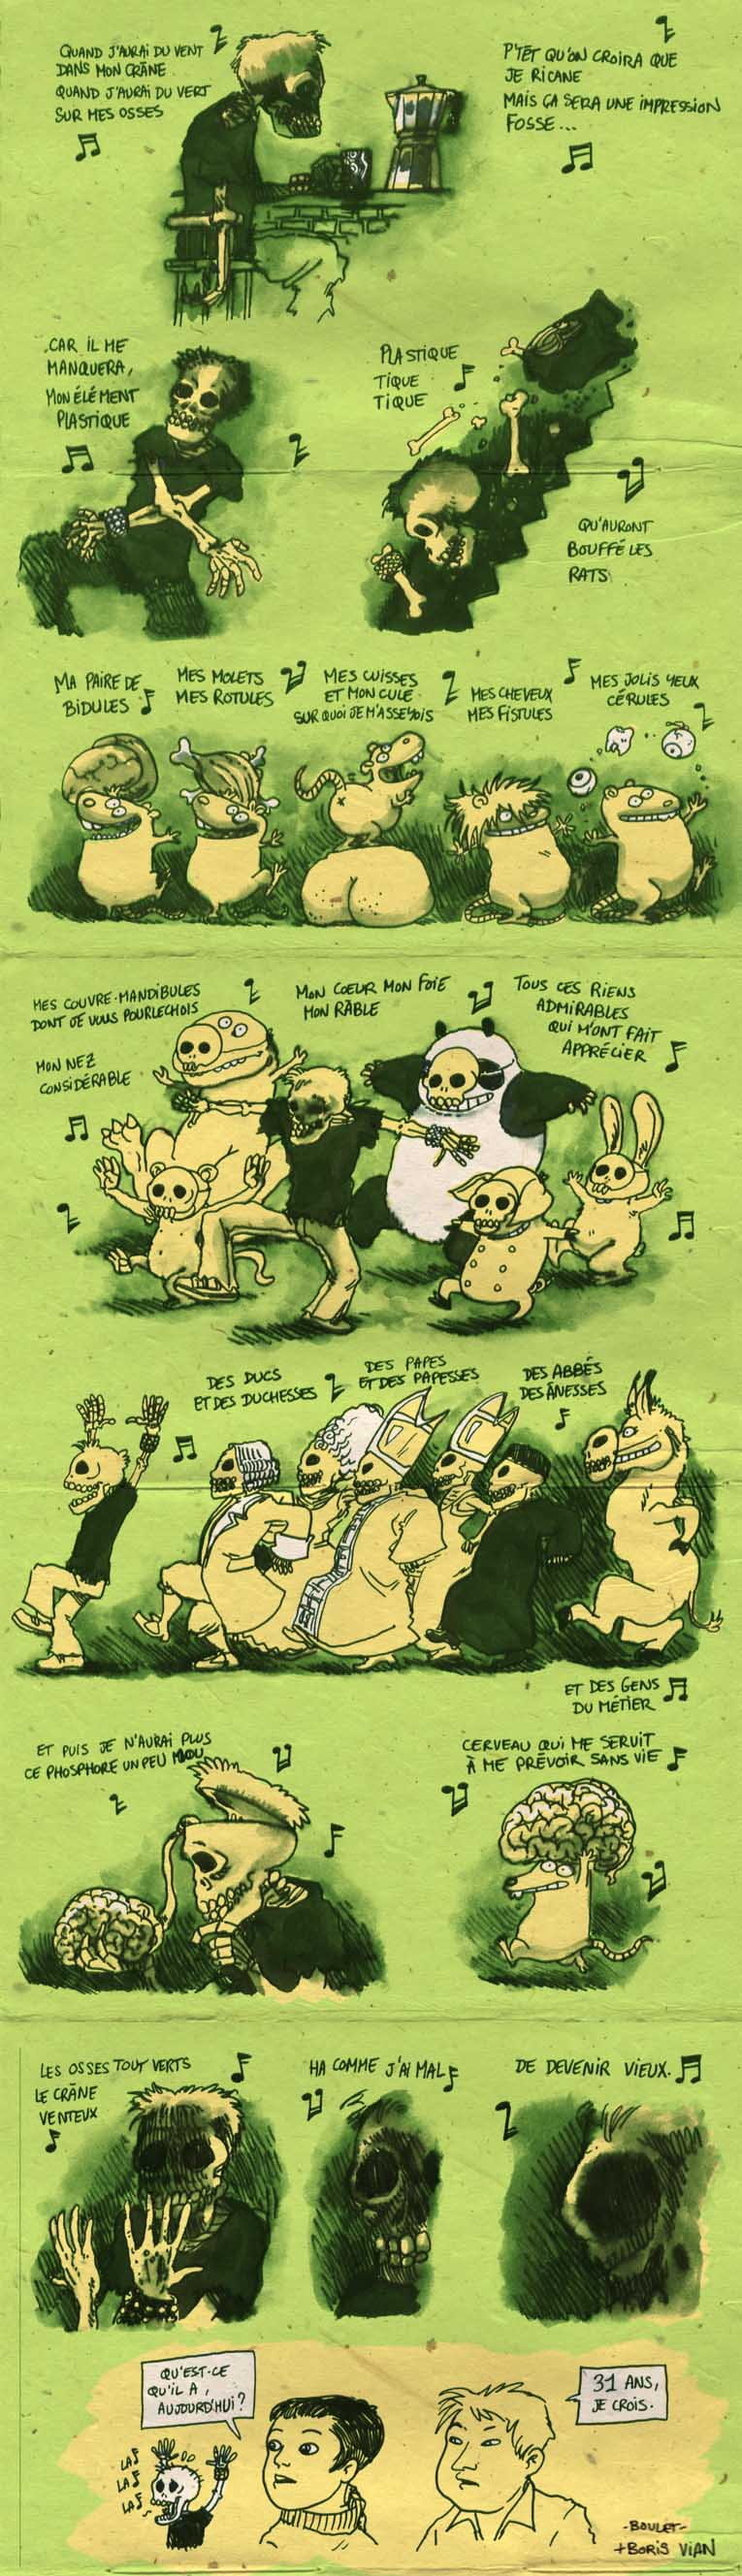
\includegraphics[trim=0cm 337mm 0cm 0cm, clip]{\PIXPATH/bouletbison}%
%\caption{Première partie}
}
\caption{\emph{Bison Ravi}, note de Boulet du \nb{31} janvier \nb{2006}}
\label{boulet}
\end{figure}
\begin{figure}[!htb]
\ContinuedFloat
\centering
\subfloat[][]{%
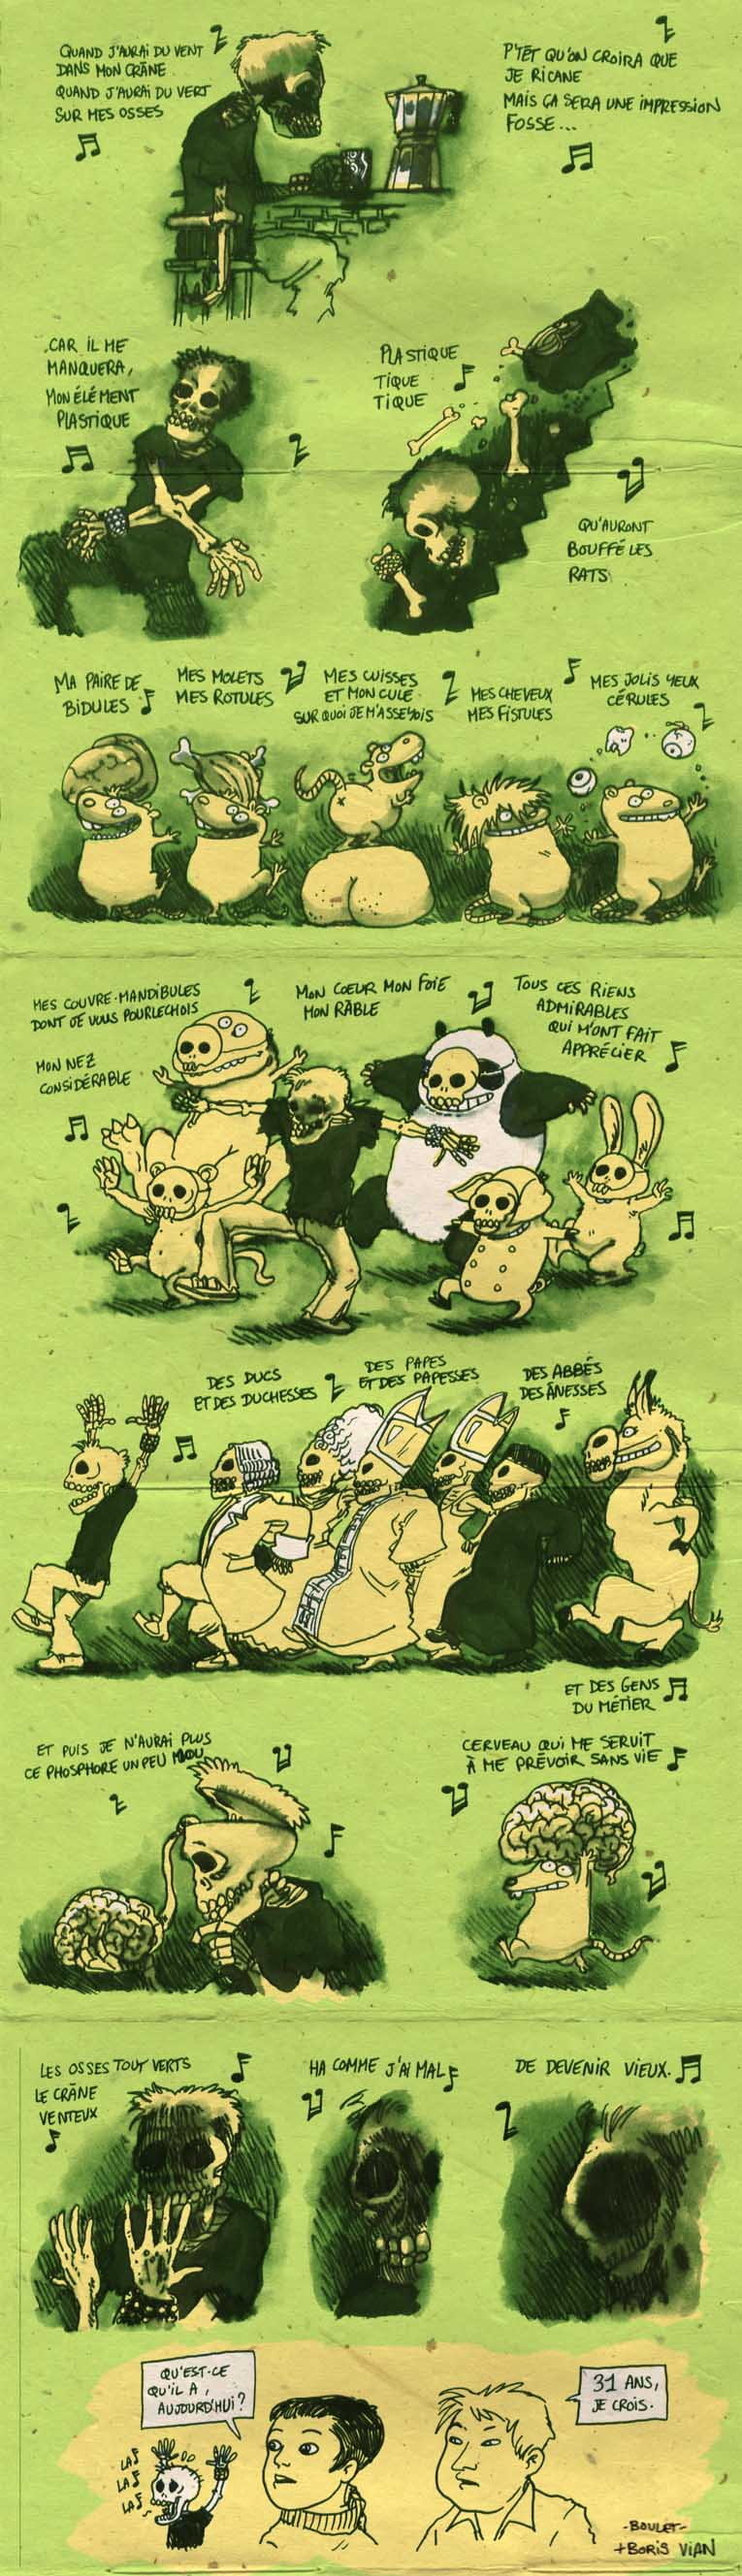
\includegraphics[trim=0cm 148mm 0cm 113mm, clip]{\PIXPATH/bouletbison}%
%\caption{Seconde partie}
}
\caption{\emph{Bison Ravi}, note de Boulet du \nb{31} janvier \nb{2006}}
\label{boulet}
\end{figure}
\eject
\begin{figure}[!htb]
\ContinuedFloat
\centering
\subfloat[][]{%
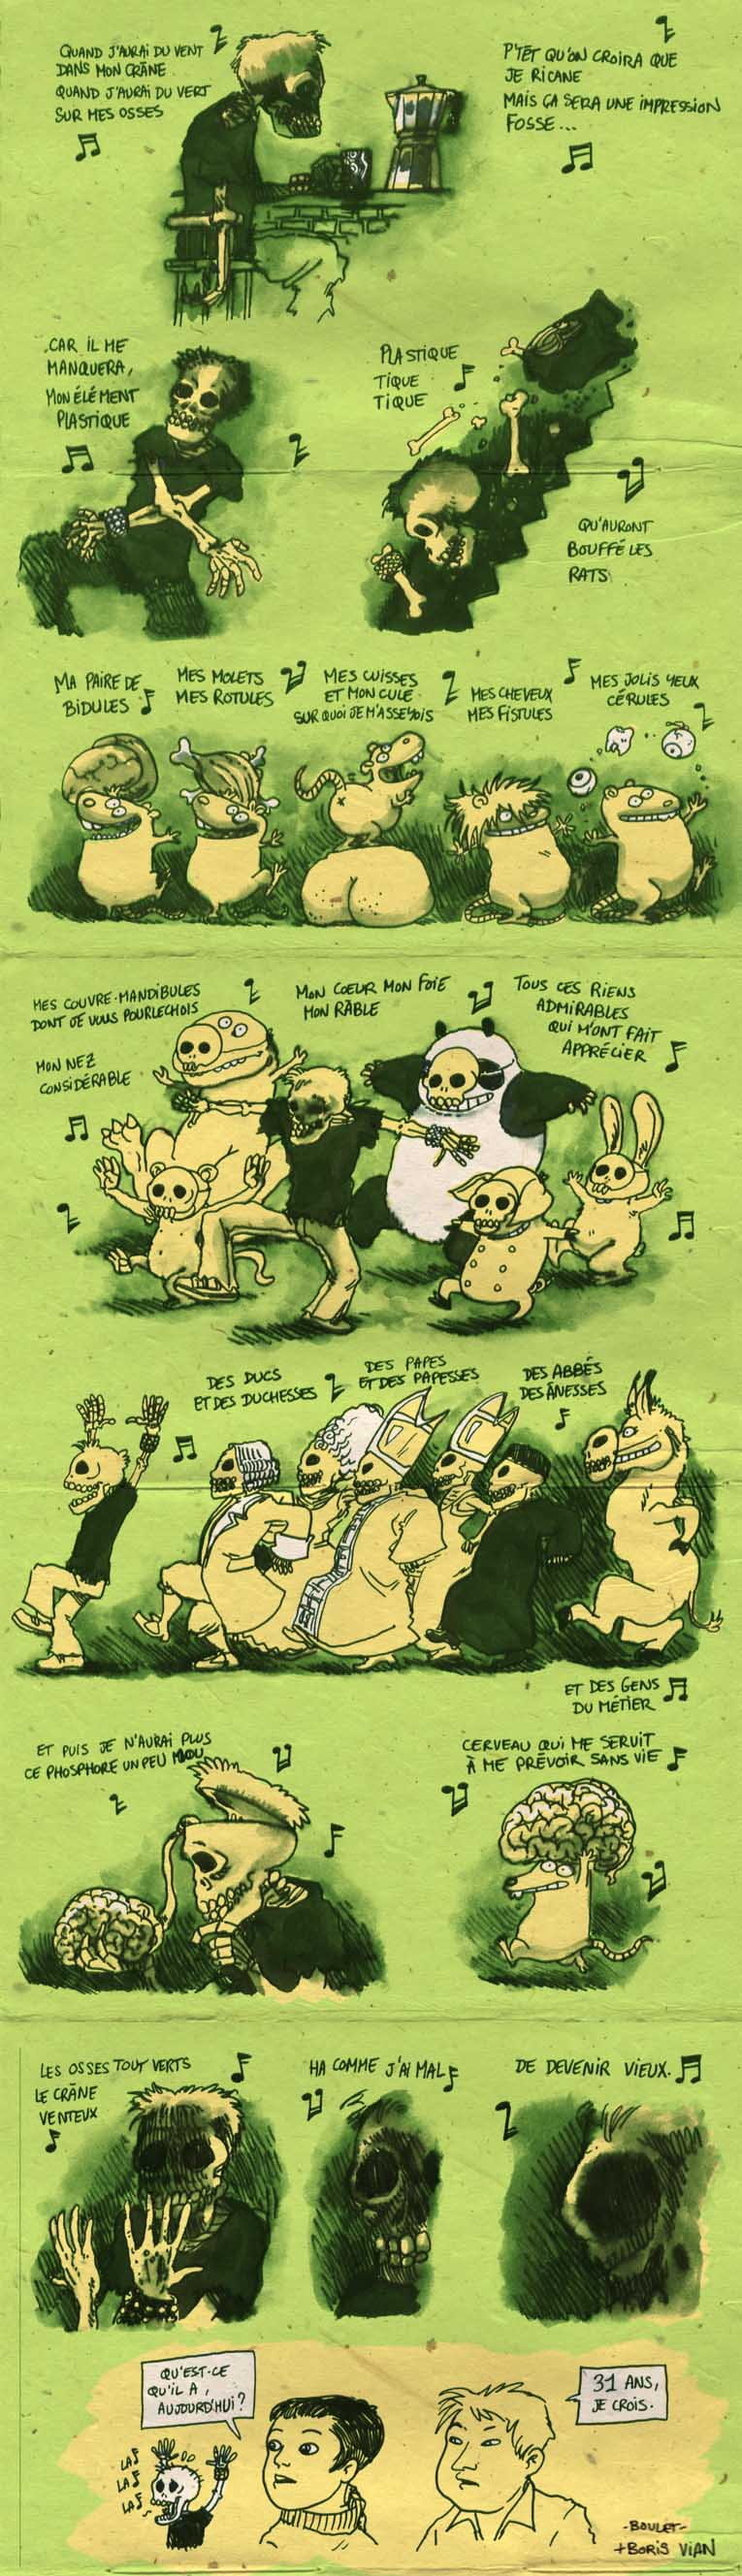
\includegraphics[trim=0cm 0mm 0cm 300mm, clip]{\PIXPATH/bouletbison}%
%\caption{Seconde partie}
}
\caption{\emph{Bison Ravi}, note de Boulet du \nb{31} janvier \nb{2006}}
\label{boulet}
\end{figure}
\eject
\FloatBarrier

\subsubsection{Je voudrais pas crever}
Il s'agit d'un poême écrit en \nb{19}??, quand il vit déjà avec Ursula
\bsc{Kubler}(son «ourson»). On ressent sans peine l'envie de vivre de
l'auteur, qui sait pertinament qu'il ne vivra pas assez longtemps pour
tout ce qu'il aimerait faire et voir.

\begin{multicols}{2}
{\footnotesize
\settowidth{\versewidth}{Où valsent les brins d'algues}
\begin{verse}
Je voudrais pas crever\\
Avant d'avoir connu\\
Les chiens noirs du Mexique\\
Qui dorment sans rêver\\
Les singes à cul nu\\
Dévoreurs de tropiques\\
Les araignées d'argent\\
Au nid truffé de bulles\\
Je voudrais pas crever\\
Sans savoir si la lune\\
Sous son faux air de thune\\
A un coté pointu\\
Si le soleil est froid\\
Si les quatre saisons\\
Ne sont vraiment que quatre\\
Sans avoir essayé\\
De porter une robe\\
Sur les grands boulevards\\
Sans avoir regardé\\
Dans un regard d'égout\\
Sans avoir mis mon zobe\\
Dans des coinstots bizarres\\
Je voudrais pas finir\\
Sans connaître la lèpre\\
Ou les sept maladies\\
Qu'on attrape là-bas\\
Le bon ni le mauvais\\
Ne me feraient de peine\\
Si si si je savais\\
Que j'en aurai l'étrenne\\
Et il y a z aussi\\
Tout ce que je connais\\
Tout ce que j'apprécie\\
Que je sais qui me plaît\\
Le fond vert de la mer\\
Où valsent les brins d'algues\\
Sur le sable ondulé\\
L'herbe grillée de juin\\
La terre qui craquelle\\
L'odeur des conifères\\
Et les baisers de celle\\
Que ceci que cela\\
La belle que voilà\\
Mon Ourson, l'Ursula\\
Je voudrais pas crever\\
Avant d'avoir usé\\
Sa bouche avec ma bouche\\
Son corps avec mes mains\\
Le reste avec mes yeux\\
J'en dis pas plus faut bien\\
Rester révérencieux\\
Je voudrais pas mourir\\
Sans qu'on ait inventé\\
Les roses éternelles\\
La journée de deux heures\\
La mer à la montagne\\
La montagne à la mer\\
La fin de la douleur\\
Les journaux en couleur\\
Tous les enfants contents\\
Et tant de trucs encore\\
Qui dorment dans les crânes\\
Des géniaux ingénieurs\\
Des jardiniers joviaux\\
Des soucieux socialistes\\
Des urbains urbanistes\\
Et des pensifs penseurs\\
Tant de choses à voir\\
A voir et à z-entendre\\
Tant de temps à attendre\\
A chercher dans le noir

Et moi je vois la fin\\
Qui grouille et qui s'amène\\
Avec sa gueule moche\\
Et qui m'ouvre ses bras\\
De grenouille bancroche

Je voudrais pas crever\\
Non monsieur non madame\\
Avant d'avoir tâté\\
Le goût qui me tourmente\\
Le goût qu'est le plus fort\\
Je voudrais pas crever\\
Avant d'avoir goûté\\
La saveur de la mort...


\end{verse}
}
\end{multicols}

J'ai intégré ce texte car je je trouve très fort et représentant bien ce sentiment de fin inéluctable et d'impuissance de \BV\ldots

J'ai pu écouter
deux très bonnes versions. La première est récitée par Jean \bsc{Rochefort} accompagné
par Claude \bsc{Luter} à la clarinette sur l'album \emph{Une heure passée avec \BV\ }
sorti en \nb{1987}; la seconde est récitée par Édouard \bsc{Baer} sur
l'album-hommage \emph{À \BV: On est pas là pour se faire engueuler !} sorti en \nb{2009}.

%\section{Un héritage riche et une influence encore vive aujourd'hui}
\section{Un héritage riche}

En ayant à l'esprit toutes (ou ne serait-ce même qu'une partie) des activités,
tous les métiers qu'il a éxercé, il aurait été bien étonnant que \BV\ ne
laisse pas une trace, ne soit pas une source d'influences pour les générations
futures.
C'est effectivement le cas. Son héritage est riche et multiple, et je vais
dévelloper ici les trois principaux aspects (il faut bien choisir) qui me semblent
les plus marquants de ces influences.

\subsection{Culture et social}

\BV\ a laissé sa marque dans le paysage culturel et social français. Déjà
de son vivant, il marquait les esprits, étant un personnage un peu hors-norme; et
certains de ces traits, en plus de ses oeuvres, sont passés à la postérité.

\paragraph{Le Prince de Saint-Germain}

\begin{wrapfigure}{r}{.5\textwidth}
\centering
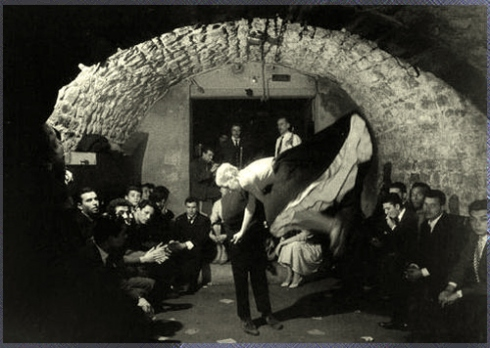
\includegraphics[width=.48\textwidth]{\PIXPATH/stgermain}
\caption{Dans une cave de St-Germain. Ici, Michelle \bsc{Vian}.}
\end{wrapfigure}
Qui n'a jamais entendu parler de Saint-Germain-des-Prés ? Je parle bien-sûr
du Saint-Germain de l'après-guerre, le lieu de rencontre des intellectuels et
des artistes parisiens: Sartre, Queneau, Prévert % TODO: citer plus
et bien d'autres. Le soir, la jeuness du tout-Paris se retrouve dans les caves
des établissements du quartier, dansant (et buvant) toute la nuit au son jazz
noir-américain. Swing, rire et cuite garantis sur facture !


\begin{wrapfigure}{l}{.5\textwidth}
\centering
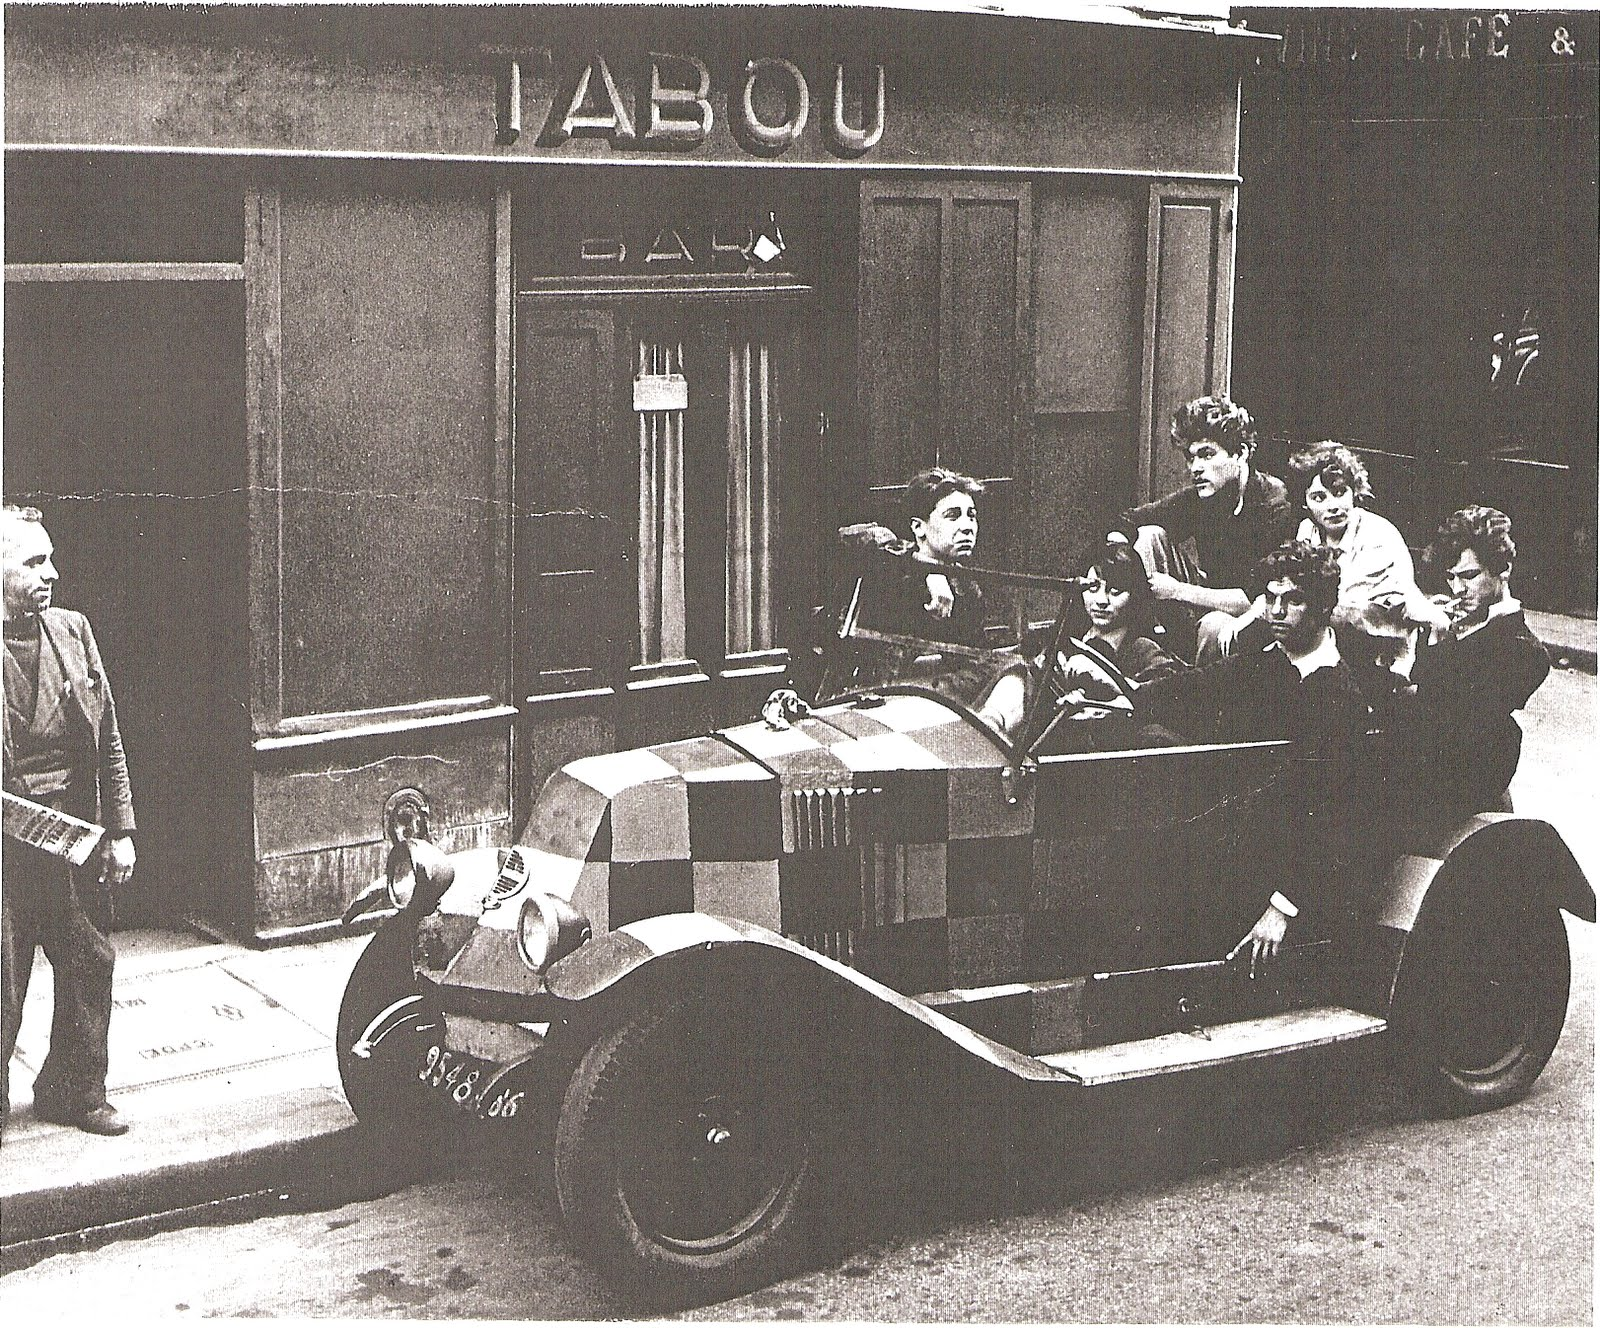
\includegraphics[width=.48\textwidth]{\PIXPATH/tabou}
\caption{Des zazous devant le Tabou.}
\end{wrapfigure}
Le surnom de «Prince de Saint-Germain» donné à \BV\ atteste de son importance
dans ce petit monde, connaissant tous (et toutes \ldots), animant avec ses amis et
ses frères les soirées endiablées, d'abord au \emph{Tabou}, puis une fois la
frénésie des premières années passées, dans l'ambiance plus feutrée du \emph{Club
Saint-Germain}.

Sa connaissance intime de Saint-Germain et de sa faune pousse un éditeur, au moment
ou Saint-Germain et les bachannales qui s'y déroulent deviennent plus connues du
grand public, de demander au «Prince» un «Guide de Saint-Germain-des-Prés».
L'ouvrage, prévu avec force descriptions farfelues et illustrations des gens et
lieux, ne fut hélas pas publié, l'éditeur ayant fait faillite entre-temps.

\begin{figure}
\centering
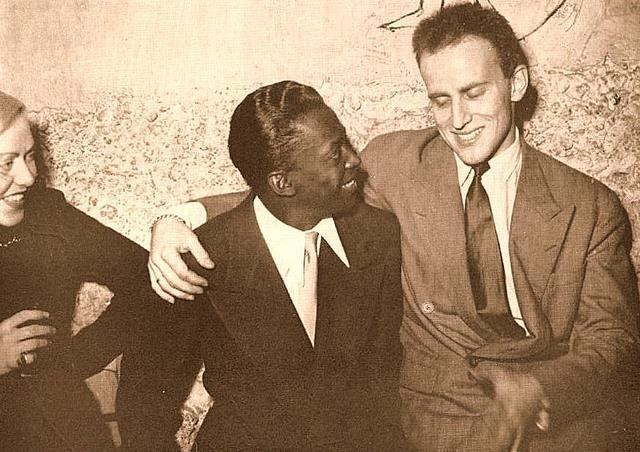
\includegraphics[width=.75\textwidth]{\PIXPATH/miles}
\caption{\BV\ et Miles \bsc{Davis}}
\end{figure}
C'est également dans ces clubs que \BV\ acceuille ses idole du jazz que sont
Miles \bsc{Davis}, Duke \bsc{Ellington} (son dieu), et bien d'autres \ldots

\paragraph{Langage}

Amateur de langage et de jeux de mots, expérimentateur du verbe et néologiste
patenté, écrivain et homme public: il n'est pas surprenant que des expressions
de son cru nous parviennent.
Le meilleur exemple est sans aucun doute l'utilisation du mot « tube ».

C'est lors d'une réunion de travail chez Philips en \nb{1957}, alors qu'il y ait
directeur artistique, qu'il propose ce mot pour désigner un succès populaire,
ou une chanson qui est assurée d'avoir du succès, parfois malgré l'ineptie du
texte ou la qualité musicale. Boris proposait ce mot pour remplacer l'alors
usité «saucisson». Devant la supériorité objective du candidat, il n'est pas
surprenant qu'il est été adopté --- difficile d'imaginer un \emph{disc jokey}
annoncer le dernier «saucisson» de l'été ! Par la même occasion, \BV\ a
fourni une alternative viable au \emph{hit} anglais. Cocorico.

\paragraph{La génération \nb{68}}

\begin{wrapfigure}{R}{.30\textwidth}
\centering

\includegraphics[width=.25\textwidth]{\PIXPATH/ecumeroumain}
\caption{Édition roumaine de \emph{L'écume des jours}. Traduction de Sorin Mărculescu}
\label{eroum}
\end{wrapfigure}
La première large reconnaissance littérarire de \BV\ --- des oeuvres signées
de son vrai nom s'entend --- fût apportée par la jeunesse de la fin des années \nb{60}.
Se sentant représentés par cet auteur si anticonformiste, anticonventionel, dont
le destin tragique à gonflé le myhte de rêveur à le jeunesse éternelle, \BV\ 
et son oeuvre --- en particulier \emph{L'écume de jours} --- ont influencé toute une
génération. En avance sur son temps comme souvent --- même lorsqu'il s'agit de
mourrir ! --- \BV\ n'a malheureusement pas connu cette gloire méritée.
Une gloire qui ne s'arrête d'ailleurs pas aux frontières de la France: \emph{L'écume
des jours} a été traduit dans plusieurs dizaines de langues, de l'anglais au japonais en passant
par le roumain (voir fig. \ref{eroum}).

\paragraph{Postérité}
Reconnu comme un auteur français incontournable, \BV\ est maintenant passé à la postérité.
Les collégiens étudient ses \oe{}uvres --- je n'ai malheureusement pas eu cette chance,
ce qui a retardé ma découverte de \BV; on trouve des établissements scolaires nommés en
son honneur (une rapide recherche Internet montre qu'il éxiste au moins 4 collèges \BV).

Sacrement suprême, son \oe{}uvre romanesque est publiée en \nb{2010} par Gallimard dans la collection
de la Pleiade. Boris rejoint ainsi le panthéon de la littérature française, \nb{50} ans après sa mort.

La Bibliothèque nationale de France à d'ailleurs, entre octobre 2011 et janvier \oldstylenums{2012}, présenté
une exposition sur BV\ (sobrement baptisée \emph{\BV}), où est retracé toute son histoire, où sont
représentées toutes ses facettes. Je n'ai malheureusement pas pu la visiter, effectuant un échange en Argentine à cette période\ldots quelle frustration ! Même si je ne regrette pour rien au monde cet échange, c'est tout de même rageant que cette évènement ait été organisé à ce moment là, j'aurais pu y consulter beaucoup de matériel pour ce PPH. Enfin, la vie est ainsi faite. Illustrée de plus de \oldstylenums{2000} documents originaux, cette
exposition montre que l'intérêt porté à \BV\ est loin de s'estomper. On pourrait même dire qu'il
grandit, en témoigne l'adaptation cinématographique de \emph{L'écume des jours} prévue pour \oldstylenums{2013}.
Réalisée par Michel \bsc{Gondry}, on pourra y voir Audrey \bsc{Tautou} donner la réplique à
Romain \bsc{Duris} et Gad \bsc{Elmaleh}. Rien que ça.

%\subsection{Musique}

%\subsection{Théâtre}


